\section{Implementation}
The program in listing \ref{lst:CUDA_EX} is additionally implemented by OpenCL, in a sequential way and multi-threaded on CPUs using OpenMP.
Execution time, initialization time and data retrieval time are measured.
Initialization time is referred to the time needed by the GPU programming models to get ready to execute the kernel function.
These steps include for instance allocating the device memory and copying of the data.
Data retrieval time contains the task to move the data back to the host memory and free the device memory.
The sizes of the matrices used in the execution are 1024 times 1024 and the mean times of 50 runs can be seen in table \ref{tab:time}.
The programs are run on a system containing an AMD Ryzen 5 1600X Six-Core processor and a GeForce RTX 2070 SUPER as GPU.
\begin{table}[htbp]
  \centering
  \caption{Initialization, Execution and Data Retrieval Time in Milliseconds of Different Implementations}
  \label{tab:time}
  \begin{tabular}{|l|c|c|c|c|}
	\hline
	  & Initialization Time & Copy Time & Execution Time & Data Retrieval Time \\\hline
	  Sequential & \texttt{-} & \texttt{-} & \(3402937.74\) & \texttt{-} \\\hline
	  Multi-Threaded & \texttt{-}& \texttt{-} & \(1126239.8\) & \texttt{-} \\\hline
	  OpenCL & \(118941.2\) & \(2072.88\) & \(3770.14\) & \(1297.68\) \\\hline
	  CUDA & \(94490.16\) & \(919.16\) & \(2591.44\) & \(1679.56\) \\\hline
  \end{tabular}
\end{table}


\begin{figure}[htbp]
  \begin{center}
  \begin{subfigure}{0.48\textwidth}
    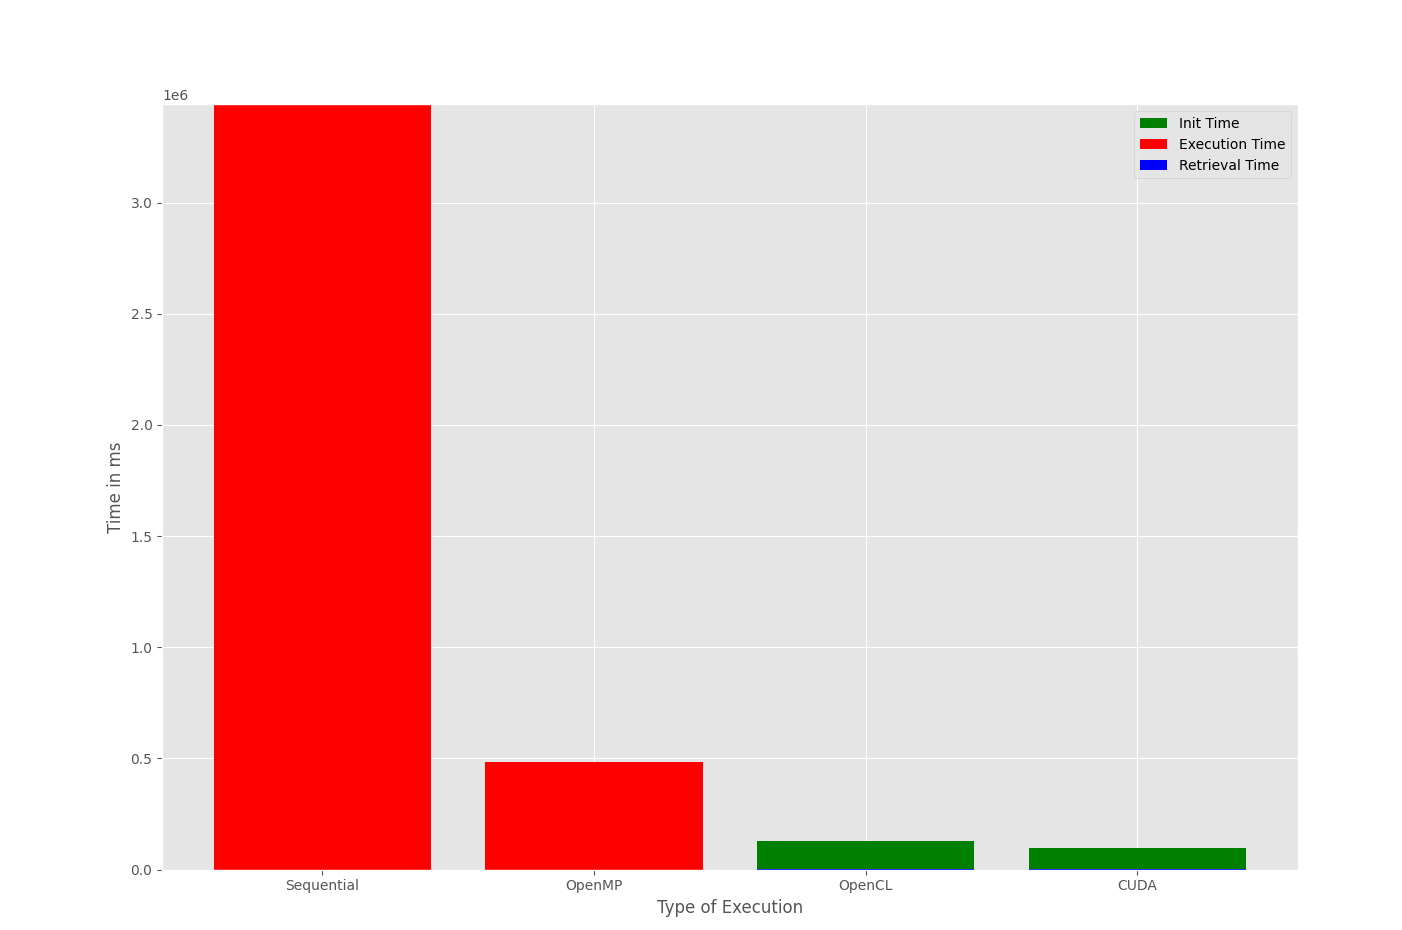
\includegraphics[width=\linewidth]{figures/results.png}
    \caption{ }
	\label{subfig:a}
  \end{subfigure}    
  \begin{subfigure}{0.48\textwidth}
    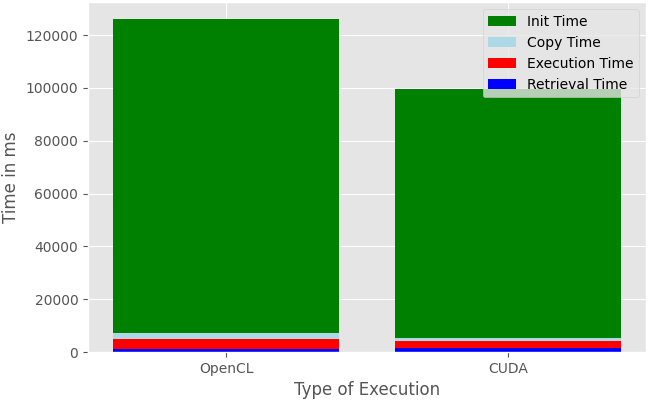
\includegraphics[width=\linewidth]{figures/GPUs_Time.png}
    \caption{ }
	\label{subfig:b}
  \end{subfigure}
    \caption{Initialization, Execution and Data Retrieval Time in Milliseconds of Different Implementations}
    \label{fig:time}
  \end{center}
\end{figure}

Figure \ref{fig:time} illustrates the ratios of time difference well.
The red parts of each bar shows the execution time needed to execute the matrix multiplication.
It can be seen that the CPU execution takes much longer than the executions using the GPU programming models --- even the multi-threaded OpenMP version using six threads.
Furthermore, subfigure \ref{subfig:b} contains only both GPU bars, so that the parts of these can be seen easier.
It shows that a lot of time is used to prepare the kernel function compared to the actual execution.

